
La población total sobre la cual se realizó el estudio es de 2388 individuos
distribuídos en 85 puntos de control. Cada punto control tiene entre 0 y 133
individuos en el estado larval con edad 0; todas las larvas tienen la misma edad
en el instante inicial de las pruebas.Además, los individuos comparten 
las mismas condiciones climáticas, es decir, la temperatura es la misma
para todos los puntos de control \\

\begin{figure}
\centering
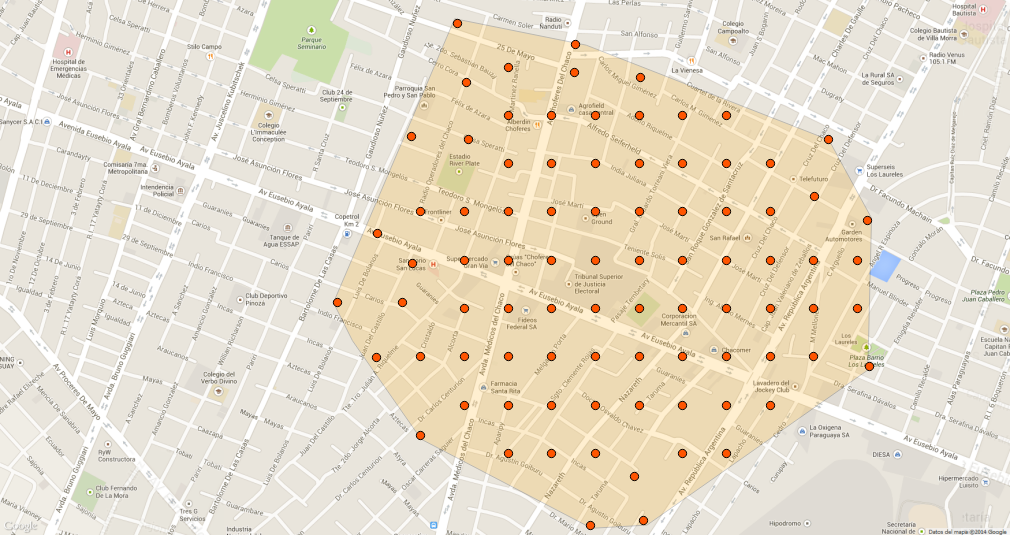
\includegraphics[width=0.9\textwidth]{./capitulo-6/graphics/puntoscontroldistribuido.png}
\caption{\label{fig:distribucion-puntos}Ubicación geográfica y distribución de puntos de control.}
\end{figure}


En la \ref{fig:distribucion-puntos} se observa la distribución de los puntos de control. Geográficamente
corresponde a 4 barrios de la ciudad de Asunción, Paraguay. Los barrios son Nazareth, 
Terminal, San Pablo e Hipódromo. Es importante aclarar que la ubicación geográfica
exacta no es relevante para el desarrollo de las pruebas, ya que no se utilizaron
condiciones climáticas propias de dicha ubicación. La ubicación geográfica sirve 
de referencia y para poder georeferenciar resultados finales. El área de covertura 
es de 2.9$km^2$ y los puntos de control se hallan ubicados uniformemente distribuidos.\\


\begin{table}
    \begin{center}
        \caption{ \label{tab:valores-formulas} Valores de parámetros en fórmulas utilizadas}
        \begin{tabular}{p{3cm} c c c c}
            \hline \\
            Variable & Simbolo & Valor & Fórmula \\
            \hline
            \hline \\
            Sitios de reproducción &  BS & 50 & ver fórmula xxx\\
            Inhibición de eclosión de huevos & $A_{0}$ & 0.5 & ver fórmula xxx\\
        \end{tabular}
    \end{center}
\end{table}
					  
La duración total de días en cada prueba es 50, se toma como día 0 el instante
inicial del proceso evolutivo y como día final al día 49. Para observar la variación
de propiedades biológicas del mosquito Aedes Aegypti se realizaron pruebas a distintas
temperaturas, dichas temperaturas se mantienen constantes durante cada prueba y son las siguientes :
15\textelsius , 18\textelsius , 20\textelsius , 22\textelsius , 
24\textelsius , 25\textelsius , 26\textelsius , 27\textelsius ,
30\textelsius , 34\textelsius \\


\subsection{Descripción general de las pruebas}

Se realizaron N iteraciones del algoritmo evolutivo y se realizaron las 
validaciones sobre el conjunto de datos generado por el mismo

Se presentan los resultados para tasa de desarroollo de las etapas inmaduras
(HUEVO, LARVA y PUPA) del Aedes Aegypti, mortalidad en cada una de las etapas,
la ovipostura, duracion del ciclo gonotrofico, alimentacion, promedio de vuelo y
desplazamiento y distribucion de sexos

\subsection{Tasa de desarollo}
Verificar las tasas de desarrollo de los individuos de la población de forma a validar
si el incremento de la madurez del individuo es correcta. Se debe contar con el tiempo
promedio de de la duración de cada estado, en días, para compararlos con los promedios
generales.

\begin{itemize}
    \item Temperatura constante
    \item Duración en promedio en cada estado a temperatura constante
    \item Desviación estándar
    \item Calcular el error
\end{itemize}

\section{Distribución de Sexo}
Se realizó un análisis para determinar la distribución del sexo del Aedes aegypti. Según
\cite{otero2006stochastic}, alrededor de la mitad de los adultos emergentes son hembras, y se
define una proporción de 1.02:1 macho: hembra. Los autores de \cite{manrique1998desarrollo} la
proporción sexual promedio de adultos emergidos es de $3$ machos por $2,75$ hembras, lo cual no representa una diferencia significativa de una relación 1:1 en las proporciones sexuales.

En general se realizaron pruebas variando la cantidad de individuos de la población, los
resultados se pueden apreciar en la tabla \tabref{tab:distribucion-sexo-test}, donde se observa que
existe una relación 1:1 para la distribución del sexo de los mosquitos.

\begin{table}
    \centering
        \caption{ \label{tab:distribucion-sexo-test} Análisis de la distribución del sexo de Aedes
        aegypti.}
        \begin{tabular}{l c c c }
            \hline \\
            Total de & Adultos & Adultos & Relación \\
            adultos  & machos  & hembras & (macho:hembra) \\
            \hline
            \hline \\
            912    &  461    &  451    &  0,99 : 1,01 \\
            1581   &  812    &  769    &  0,97 : 1,03 \\
            4154   &  2084   &  2070   &  1    : 1 \\
            9722   &  4940   &  4782   &  0,98 : 1,02 \\
            9045   &  4472   &  4573   &  1,01 : 0,99 \\
            16248  &  8104   &  8144   &  1    : 1 \\
            30693  &  15418  &  15275  &  1    : 1 \\
            28411  &  14224  &  14187  &  1    : 1 \\
        \end{tabular}
\end{table}

\section{Ciclo gonotrófico}
Para el análisis de la tasa de desarrollo, en días, del ciclo gonotrófico de las hembras del Aedes
aegypti, se clasificó la población en hembras núliparas y paridas. En la
\tabref{tab:ciclo-gonotrofico-test} se puede observar una media de $5,03$ días para las hembras
nulíparas y  $2,92$ días para las paridas para una temperatura aproximada de $25,11$ \textcelsius.

\begin{table}[!htbp]
    \begin{minipage}{\textwidth}
        \centering
        \caption{ \label{tab:ciclo-gonotrofico-test} Análisis de duración del ciclo gonotrófico
        de la hembra de Aedes aegypti nueve temperaturas constantes  (18-34 \textcelsius).}
        \begin{tabular}{l *{10}{c} }
            \hline \\
            & &  & &  & &  &  &  &  & Media\\
            Población & 18\textcelsius & 20 \textcelsius & 22 \textcelsius & 24 \textcelsius
                      & 25 \textcelsius & 26\textcelsius  & 27 \textcelsius & 30 \textcelsius
                      & 34\textcelsius & General\\

            \hline
            \hline \\
            Nulíparas\footnote{Hembras nulíparas que no han ovipuesto.}
                        & 8,97 & 7,4  & 6,13  & 5,08  & 4,63 & 4,22  & 3,85 & 2,94 & 2,06 & 5,03\\
            Paridas\footnote{Hembras que ya han realizado al menos una ovipostura.}
                        & 5,21 & 4,3  & 3,56  & 2,95  & 2,69 & 2,45  & 2,24 & 1,71 & 1,2 & 2,92\\
            Media \footnote{Promedio general de la duración general del ciclo gonotrófico para las
            hembras}
                        & 7,09 & 5,85 & 4,85  & 4,02  & 3,66 & 3,34  & 3,05 & 2,33 & 1,63 & 3,98\\
        \end{tabular}
    \end{minipage}
\end{table}

Las variaciones en la temperatura influyen en tiempo de digestión de la sangre y el
desarrollo de los ovarios, a medida que la temperatura desciende, la digestión y por ende el ciclo
gonotrófico tomará más tiempo (\figref{fig:ciclo-gonotrofico-temperatura}). En \cite{edman1987host}
se observó que hembras nulíparas de Aedes aegypti poseen un proceso de digestión es más lento en
las hembras paridas y por ende el ciclo gonotrófico de las mismas tiene a ser más largo. Existen
diversos estudios, que han reportado que el patrón diario de alimentación de los mosquitos, varia
de acuerdo a las localidades y subespecies. A continuación se mencionaran algunos estudios
realizados correspondientes a la duración del ciclo gonotrófico, con el fin de realizar una
comparación con los resultados obtenidos mediante el proceso evolutivo.

\begin{figure}[!htbp]
    \centering
    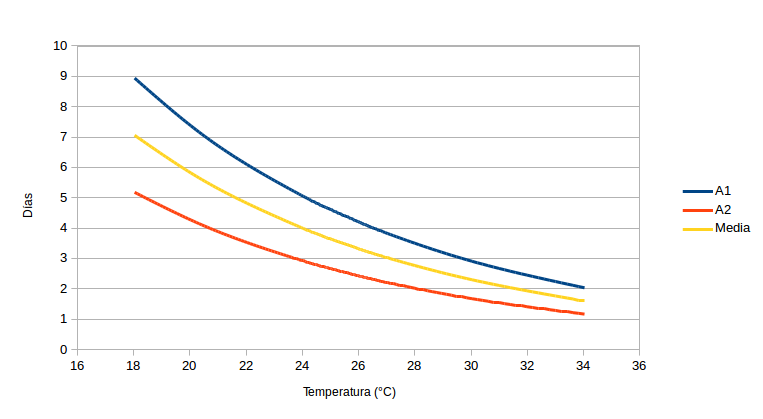
\includegraphics[width=1\textwidth]{capitulo-6/graphics/ciclo-gonotrofico-temperatura.png}
    \caption{\label{fig:ciclo-gonotrofico-temperatura} Tasa de desarrollo, en días, del ciclo
    gonotrófico de hembras nulíparas, hembras paridas y la media general a nueve temperaturas
    constantes (18-34 \textcelsius).}
\end{figure}

En \cite{beltran2001bionomia} se determinó que la duración del ciclo gonotrófico del Aedes
aegypti, para los siguientes municipios de México en, 3 días para Tamazula de Gordiano a una
temperatura de $21,5$ \textcelsius, 3 días para Techaluta de Montenegro a $22,8$ \textcelsius, 4
días para Tuxpan a 22 \textcelsius y 5 días para CD Zacoalco de Torres a $22,7$ \textcelsius.

En \cite{luevano1993ciclo}, el autor determinó la duración del ciclo gonotrófico de las
poblaciones naturales de Aedes aegypti en el área metropolitana de Monterrey, Nuevo León. México,
en cinco días, a una temperatura promedio de $25,5$ \textcelsius.

En \cite{trpis1986dispersal} los autores reportaron una duración del ciclo gonotrófico en Kenia a
nivel rural de, 5 a 7 días para el primer ciclo (hembras nulíparas) y de 4 a 5 días para los
siguientes ciclos (hembras paridas). El método utilizado fue de captura con cebo humano de
mosquitos de Aedes aegypti.

Según \cite{sivanathan2006ecology} el ciclo gonotrófico del aAedes aegypti y Aedes albopictus se
encuentra acotada entre $2,73$ a 3 días respectivamente.

Las diferentes condiciones climáticas y la capacidad de adaptación en habitad específicos, del
Aedes aegypti, son las responsables de diferencias que se puedan tener entre cepas del mosquito.
La duración del ciclo gonotrófico obtenida, depende de los coeficientes para el modelo de
maduración enzimática de \cite{sharpe1977reaction} que fue tomado de \cite{otero2006stochastic},
que según los autores fue tomado de \cite{focks1993dynamic}.


\section{Ovoposturas}
Como se menciona en la la sección \ref{subsec:cap4-oviposicion} la cantidad de huevos generados,
por una hembra, se encuentra definida como una constante independiente de la temperatura temperatura de valor 63. En la tabla
\ref{tab:ovipostura-cantidad-test} se presentan los resultados obtenidos de la cantidad de
huevos generados. En general fueron generados 747739 huevos por 11708 hembras adultas dejando
un promedio de 63.87 huevos por hembra, dejando un error 0.87 huevos.

\begin{table}
    \begin{center}

        \caption{ \label{tab:ovipostura-cantidad-test} Análisis de la
        cantidad de huevos de Aedes Aegypti generados a diez temperaturas
        constantes  (15-34 \textcelsius).}
        \begin{tabular}{p{3cm} c c  }
            \hline \\
            Temperatura  & Cantidad          & Cantidad \\
            \textcelsius & de oviposiciones  & de huevos \\
            \hline
            \hline \\
                15 & 0    & 0\\
                18 & 44   & 2772\\
                20 & 91   & 5733\\
                22 & 119  & 7497\\
                24 & 431  & 27153\\
                25 & 810  & 51030\\
                26 & 1003 & 63189\\
                27 & 1185 & 74655\\
                30 & 5206 & 327978\\
                34 & 2058 & 129654\\

        \end{tabular}
    \end{center}
\end{table}


\section{Vuelo y dispersión}
Para el análisis de la distancia recorrida, en metros, del adulto de Aedes aegypti, se realizaron
pruebas a 9 temperaturas constantes (15-34\textcelsius), solo las hembras que han ovipuesto al
menos una vez fueron incluidas. En la tabla \ref{tab:pomedio-vuelo-test} se presentan los
resultados obtenidos para la disperción de las hembras adultas del aedes aegypit agrupadas por el
tipo su tipo de zona, en general se obtuvo un promedio de $65,74$, $63,97$ $1308,19$ metros para las zonas buena, normal y malas respectivamente. Existen diversos estudios, que han reportado que
la disperción del aedes aegypti en relación a las caracteristicas de su ambiente. A continuación
se mencionaran algunos estudios realizados, con el fin de realizar una comparación con los resultados obtenidos.

En \cite{cabezas2005dengue} señalan que por lo general mosquito no sobrepasa los 50 a 100 metros
durante su vida, ya que tiende a permanecer en el lugar donde emergió.

Según \cite{ThironIzcazaJ2003} por lo general, la hembra de Ae. aegypti, permanece físicamente en
donde emergió, siempre y cuando no halla algún factor que la perturbe o no disponga de huéspedes,
sitios de reposo y de postura. En caso de no haber recipientes adecuados, la hembra grávida es capaz de volar hasta tres kilómetros en busca de este sitio.

Los autores de \cite{dengueUruguayCap8} señalan que, para las estrategias de control de Aedes
aegypti en zonas urbanas donde existen brotes de dengue y fiebre amarilla se asume que los
mosquitos tienen un rango de vuelo durante su vida de 50 a 100 metros.

En \cite{luevano1993ciclo} se reporta, que el aedes aegypti es un mosquito doméstico que
generalmente esta confinado a las casas donde se cria, tiene un rango de vuelo corto, entre 23 a 50 metros, y raramente se dispersa a largas distancias.

\cite{mcdonald1977population} en Kenia, liberó poblaciones de Aedes aegypti a las distancias de,
200, 400 y 800 metros, y observó que aproximadamente el 50 \% de los mosquitos marcados se
dispersaron a 200 metros del punto en el cual fueron liberados, un 10 \% a 400 metros y solamente
el 1 \% se dispersó a 800 metros.

En \cite{trpis1986dispersal}, los autores reportaron que en Kenia, que la tasa media de dispersión
de las hembras fue de 57 metros. La distancia máxima de las hembras durante 24 horas fue de 154
metros.

La mayoría de los estudios coinciden que, los adultos del aedes aegypti, en condiciones óptimas de
disponibilidad de alimento y sitios adecuados de ovipostura, tienden a permanecer en el lugar
donde emergieron, con una dispersión media estimada entre 50 y a 100 metros, su presencia es
prácticamente un indicio certero de la proximidad de los criaderos. En caso de no contar con
sitios adecuados de ovipostura y disponibilidad de alimento tienden a dispersarme una mayor
distancia en busca de mejores condiciones.

\begin{table}
    \begin{minipage}{\textwidth}
        \caption{ \label{tab:pomedio-vuelo-test} Análisis de la dispersión, por zona, del adulto
        de Aedes aegypti diez temperaturas constantes (15-34 \textcelsius).}
        \begin{tabular}{p{4cm} *{4}{c}  }
          \hline \\
          Temperatura (\textcelsius)& Buena & Normal & Mala & Media Obtenida\\
          \hline
          \hline \\
          18 & 89,06 & 66,61 & 1274,97 & 476,88\\
          20 & 66,52 & 73,53 & 1516,43 & 552,16\\
          22 & 77,89 & 63,78 & 1003,9 & 381,86\\
          24 & 60,28 & 62,31 & 1077,6 & 400,06\\
          25 & 54,52 & 63,66 & 1397,31 & 505,16\\
          26 & 61,61 & 60,79 & 1509,67 & 544,02\\
          27 & 65,24 & 63,72 & 1433,58 & 520,85\\
          30 & 62,61 & 59,56 & 1213,1 & 445,09\\
          34 & 53,92 & 61,75 & 1347,13 & 487,6\\
          Media General & 65,74 & 63,97 & 1308,19 & 479,3\\
        \end{tabular}
    \end{minipage}
\end{table}

 
